\documentclass[11pt,class=report,crop=false]{standalone}
\usepackage[screen]{../python}

\begin{document}

%====================================================================
\chapitre{Random blocks}
%====================================================================

\objectifs{You will program two methods to build figures that look like algae or corals. Each figure is made up of small randomly thrown blocks that stick together.}

\begin{center}
\begin{minipage}{0.4\textwidth}
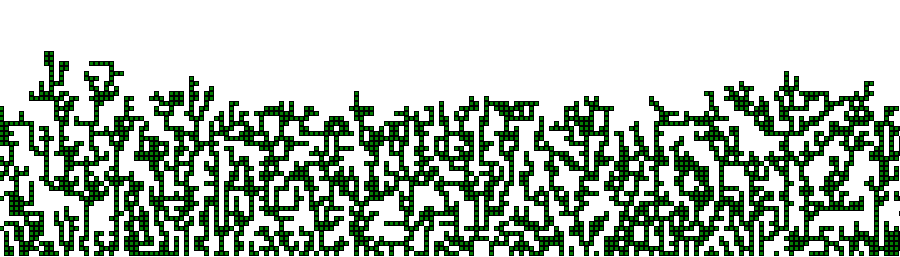
\includegraphics[scale=\myscale,scale=0.3]{screen-blocks-bloc00}
\end{minipage}
\begin{minipage}{0.3\textwidth}
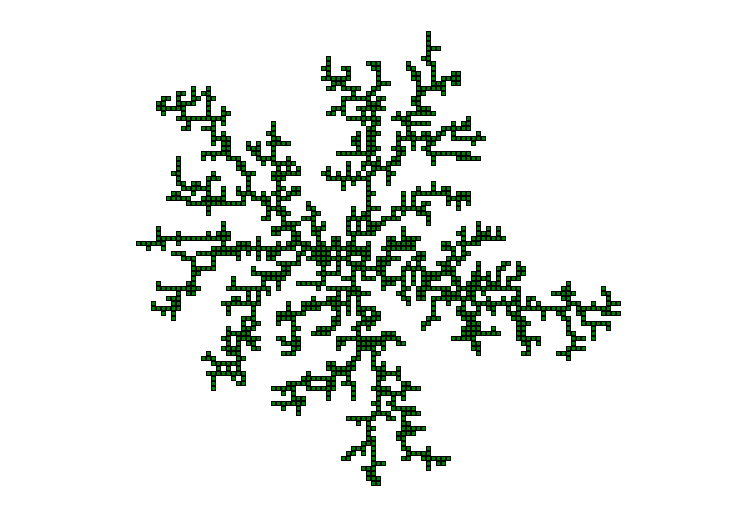
\includegraphics[scale=\myscale,scale=0.25]{screen-blocks-tree00}
\end{minipage}
\end{center}



%%%%%%%%%%%%%%%%%%%%%%%%%%%%%%%%%%%%%%%%%%%%%%%%%%%%%%%%%%%%%%%%
%%%%%%%%%%%%%%%%%%%%%%%%%%%%%%%%%%%%%%%%%%%%%%%%%%%%%%%%%%%%%%%%

\begin{cours}[Fall of blocks]
Square blocks are dropped into a grid, on the principle of the game \og{}Connect 4\fg{}: after choosing a column, a block falls from top to bottom. The blocks are placed on the bottom of the grid or on other blocks or next to other blocks. There is a big difference with the game \og{}Connect 4\fg{}, here the blocks are \og{}sticky\fg{}, i.e. a block stays stuck as soon as it meets a neighbor on the left or right.


Here is an example of how to throw blocks:
\myfigure{0.5}{
\footnotesize
  \tikzinput{fig-blocks-0}
}

For example, in step 4, the block thrown in the column $2$ does not go down to the bottom but remains hung on its neighbor, so it is permanently suspended.

The random throwing of hundreds of blocks on a large grid produces pretty geometric shapes resembling algae.

\begin{center}
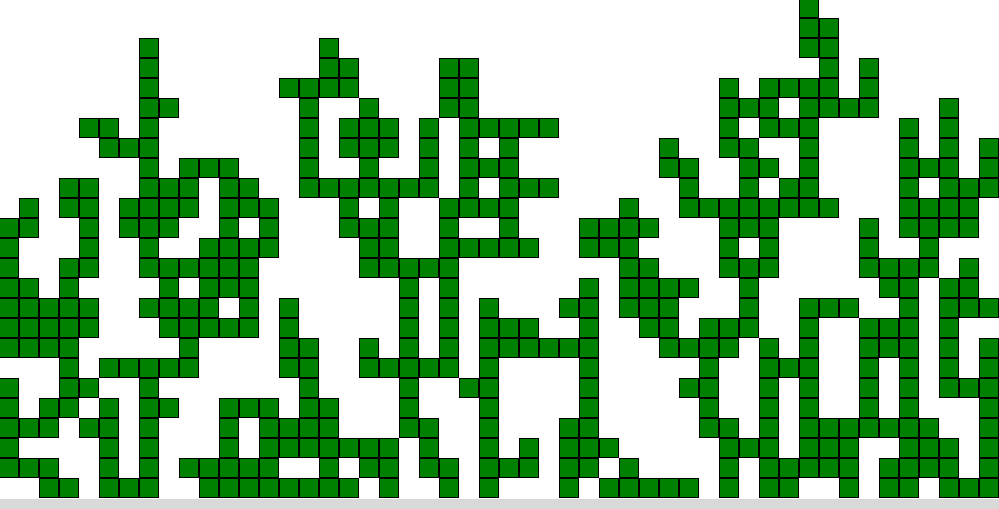
\includegraphics[scale=\myscale,scale=0.3]{screen-blocks-bloc0}
\end{center}

\end{cours}



%%%%%%%%%%%%%%%%%%%%%%%%%%%%%%%%%%%%%%%%%%%%%%%%%%%%%%%%%%%%%%%%
% Activity 1 - Block falls
%%%%%%%%%%%%%%%%%%%%%%%%%%%%%%%%%%%%%%%%%%%%%%%%%%%%%%%%%%%%%%%%

\begin{activite}[Fall of blocks]

\objectifs{Goal: program the drop of the blocks (without graphic display).}

The workspace is modeled by an array of $n$ rows and $p$ columns. At the beginning the array only contains $0$'s;
 then the presence of a block is represented by $1$.

Here is how to initialize the table:
\mycenterline{\ci{array = [[0 for j in range(p)] for i in range(n)]}}
The table is modified by instructions of the type:
\mycenterline{\ci{array[i][j] = 1}}


Here is an example of a table (left) to represent the graphical situation on the right (the block at the top right is falling).

\begin{center}
\begin{minipage}{0.3\textwidth}
$$\begin{array}{cccccc}
0&0&0&0&1&0\\
0&0&1&0&0&0\\
0&0&1&0&0&0\\
0&0&1&1&0&0
\end{array}$$
\end{minipage}
\begin{minipage}{0.4\textwidth}
\myfigure{0.7}{
  \tikzinput{fig-blocks-1}
}
\end{minipage}
\end{center}

\begin{enumerate}
  \item Program a function \ci{can_fall(i,j)} that determines if the block in position $(i,j)$ can drop to the square below or not.
  
  Here are the cases in which the block \emph{cannot} fall:
  \begin{itemize}
    \item if the block is already on the last line,
    \item if there is a block just below,
    \item if there is a block just to the right or just to the left.
  \end{itemize}
  
  \item Program a function \ci{drop_one_block(j)}
which drops a block in the $j$ column until it can no longer go down.
This function modifies the array.  
  
  For example, here is the table before (left) and after (right) dropping a block in the $j=3$ column.  
  
$$\begin{array}{cccccc}
0&0&0&0&0&0\\
0&0&1&0&0&0\\
0&0&1&0&0&0\\
0&0&1&1&0&0
\end{array}\qquad\qquad
\begin{array}{cccccc}
0&0&0&0&0&0\\
0&0&1&1&0&0\\
0&0&1&0&0&0\\
0&0&1&1&0&0
\end{array}
$$
 
 \myfigure{0.7}{
  \tikzinput{fig-blocks-2}
} 

 
  \item Program a function \ci{drop_blocks(k)} that launches 
  $k$ blocks one by one, each time choosing a random column (i.e. an integer $j$ with $0 \le j < p$). 
  
  Here is an example of a table obtained after throwing $10$ blocks:
  
 
\begin{center}
\begin{minipage}{0.3\textwidth} 
 $$\begin{array}{cccccc} 
0&0&0&1&1&0\\
0&1&1&1&0&0\\
0&0&1&0&0&1\\
0&0&1&1&0&1
\end{array}
$$
\end{minipage}
\begin{minipage}{0.4\textwidth} 
 \myfigure{0.7}{
  \tikzinput{fig-blocks-3}
} 
\end{minipage}
\end{center}  

\end{enumerate}

\end{activite}


%%%%%%%%%%%%%%%%%%%%%%%%%%%%%%%%%%%%%%%%%%%%%%%%%%%%%%%%%%%%%%%%
% Activity 2 - Falling blocks
%%%%%%%%%%%%%%%%%%%%%%%%%%%%%%%%%%%%%%%%%%%%%%%%%%%%%%%%%%%%%%%%

\begin{activite}[Falling blocks (continued)]

\objectifs{Goal: program the graphic display of the blocks.}

\textbf{Static display.} Program the graphical display of blocks from an array.

\begin{center}
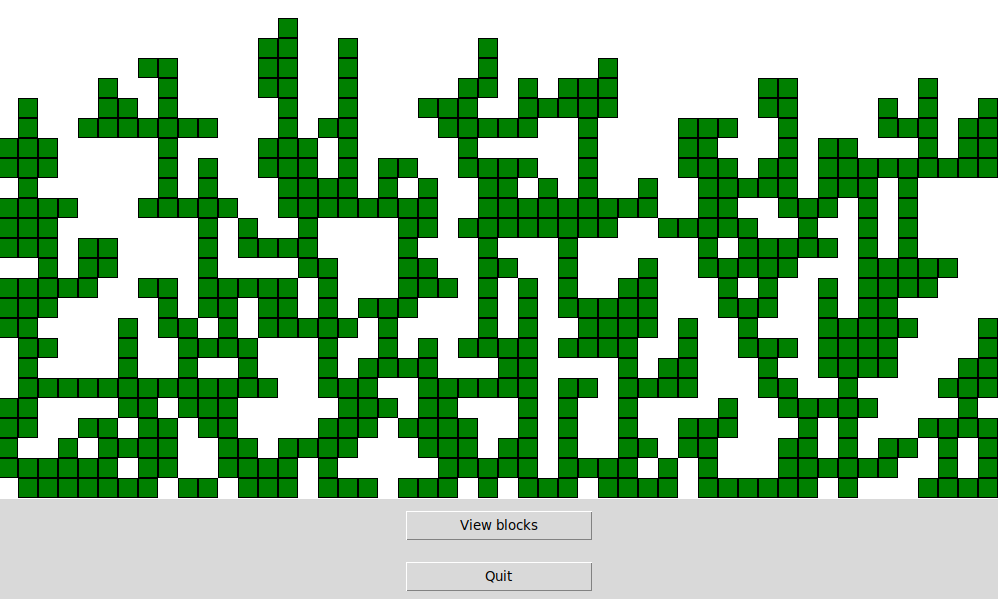
\includegraphics[scale=\myscale,scale=0.3]{screen-blocks-bloc1-en}
\end{center}
\medskip

\emph{Hints.}
\begin{itemize}
  \item Use the module \ci{tkinter}, see chapter \og{}Statistics -- Data visualization\fg{}.
  \item You can add a button that launches a block (or several at once). 
\end{itemize}

\medskip



\textbf{Dynamic display (optional and difficult).} Program the display of falling blocks.
\medskip

\begin{center}
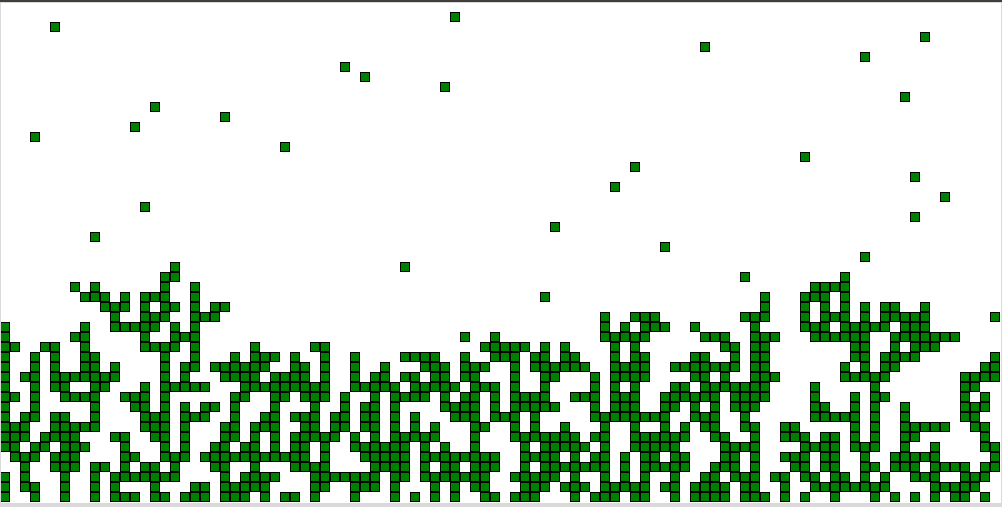
\includegraphics[scale=\myscale,scale=0.3]{screen-blocks-bloc2}
\end{center}

\emph{Hints.} 
\begin{itemize}
  \item It's much more complicated to program, but very nice to see! 
  \item For moving the blocks, use the program \og{}Moves with \ci{tkinter}\fg{} at the end of this chapter.
  \item How to make a \og{}block rain\fg{}? On a regular basis (for example every tenth of a second) all existing blocks are dropped by one square and a new one appears on the top line.
\end{itemize}
\end{activite}





%%%%%%%%%%%%%%%%%%%%%%%%%%%%%%%%%%%%%%%%%%%%%%%%%%%%%%%%%%%%%%%%
%%%%%%%%%%%%%%%%%%%%%%%%%%%%%%%%%%%%%%%%%%%%%%%%%%%%%%%%%%%%%%%%

\begin{cours}[Brownian trees]

Here is a slightly different construction, much longer to calculate, but which also draws pretty figures called \og{}brownian trees\fg{}.

\begin{center}
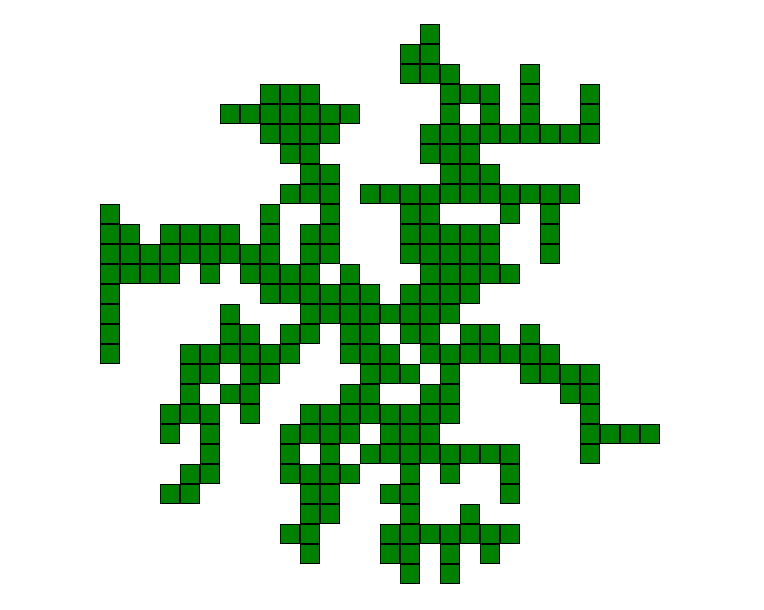
\includegraphics[scale=\myscale,scale=0.28]{screen-blocks-tree1}
\end{center}


The principle is as follows:
\begin{itemize}
  \item We start from a grid (this time we have to imagine that it is drawn flat on a table). In its center, we place a first fixed block, the \emph{seed}.
  
  \item A random new block is created on the grid. At each step, this block moves at random to one of the eight adjacent squares, we are talking about a \emph{brownian movement}. 

  \item As soon as this block touches another block from one side, it sticks to it and no longer moves.

  \item If the block leaves the grid, it disintegrates.
  
  \item Once the block has been glued or disintegrated, a new block is then restarted from a random point on the grid.
\end{itemize}


\myfigure{0.5}{
\footnotesize
  \tikzinput{fig-blocks-tree1}
} 

Gradually, we obtain a kind of tree that looks like coral. The calculations are very long because many blocks come out of the grid or take a long time to fix (especially at the beginning). In addition, the blocks can only be thrown one by one.

\end{cours}



%%%%%%%%%%%%%%%%%%%%%%%%%%%%%%%%%%%%%%%%%%%%%%%%%%%%%%%%%%%%%%%%
% Activity 3 - Brownian trees
%%%%%%%%%%%%%%%%%%%%%%%%%%%%%%%%%%%%%%%%%%%%%%%%%%%%%%%%%%%%%%%%

\begin{activite}[Brownian trees]

\objectifs{Goal: program the creation of a brownian tree.}

\textbf{Part 1.}

\begin{enumerate}
  \item Model the workspace again with an array of $n$ rows and $p$ columns containing $0$ or $1$. Initialize all values to $0$, except $1$ in the center of the table.
  
  \item Program a function \ci{is_inside(i,j)} which determines if the position $(i,j)$ is in the grid (otherwise the block is coming out).
    
  \item Program a function \ci{can_move(i,j)} that determines if the block in position $(i,j)$ can move (the function returns \og{}True\fg{}) or if it is hung on (the function returns \og{}False\fg{}).

  \item Program a function \ci{launch_one_block()}, without parameters, that simulates the creation of a block and its random movement, until it sticks or leaves the grid.
  
  \emph{Hints.}
  \begin{itemize}
    \item The block is created at a random position $(i,j)$ of the grid.
    \item As long as the block is in the grid and free to move:
    \begin{itemize}
      \item you choose a horizontal move by randomly drawing an integer from $\{-1,0,+1\}$, the same for a vertical move;
      \item you move the block according to the combination of these two movements.
    \end{itemize}  
    \item Then modify the table.      
  \end{itemize}

  
    \item End with a function \ci{launch_blocks(k)} that launches $k$ blocks.   
\end{enumerate}


\textbf{Second part.}

Program the graphic display using \ci{tkinter}. You can add a button that launches $10$ blocks at once.

\begin{center}
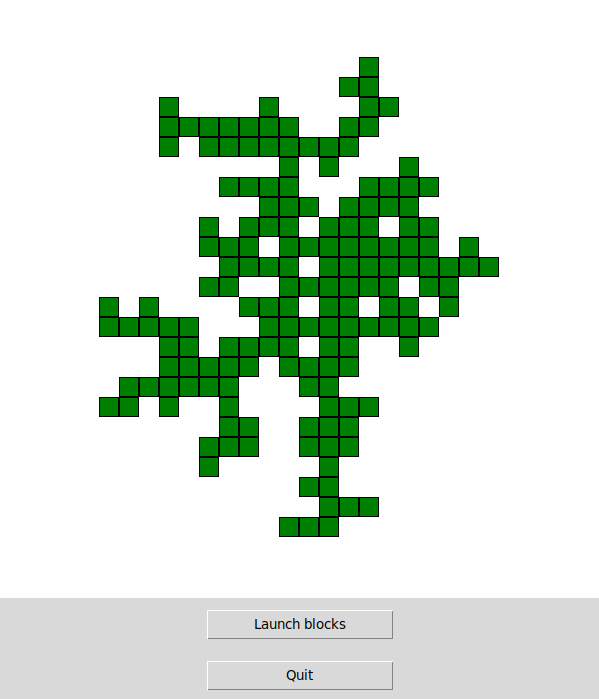
\includegraphics[scale=\myscale,scale=0.30]{screen-blocks-tree2-en}
\end{center}

\end{activite}


%%%%%%%%%%%%%%%%%%%%%%%%%%%%%%%%%%%%%%%%%%%%%%%%%%%%%%%%%%%%%%%%
%%%%%%%%%%%%%%%%%%%%%%%%%%%%%%%%%%%%%%%%%%%%%%%%%%%%%%%%%%%%%%%%


\begin{cours}[Moves with \og{}tkinter\fg{}]

\index{tkinter@\ci{tkinter}}
\index{module!tkinter@\ci{tkinter}}

Here is a program that moves a small square and bounces it off the edges of the window.

\begin{center}
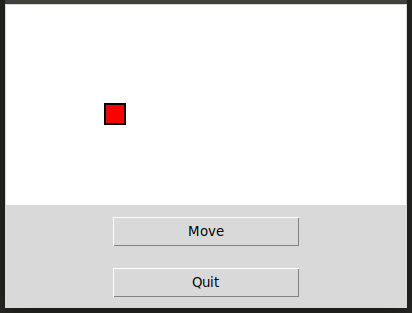
\includegraphics[scale=\myscale,scale=0.5]{screen-blocks-lesson-move-en}
\end{center}

Here are the main points:
\begin{itemize}
  \item An object \ci{rect} is defined, it is a global variable, as well as its coordinates \ci{x0}, \ci{y0}.
  
  \item This object is (a little bit) moved by the function \ci{mymove()} which shifts the rectangle by \ci{(dx,dy)}.
    
  \item The key point is that this function will be executed again after a short period of time. The command: 
  \mycenterline{\ci{canvas.after(50,mymove)}}  
  requests a new execution of the function \ci{mymove()} after a short delay (here $50$ milliseconds).
  
  \item The repetition of small shifts simulates movement.
\end{itemize}

\begin{lstlisting}
from tkinter import *

the_width = 400
the_height = 200

root = Tk()     
canvas = Canvas(root, width=the_width, height=the_height, background="white")
canvas.pack(fill="both", expand=True)

# Coordinates and speed
x0, y0 = 100,100
dx = +5  # Horizontal speed
dy = +2  # Vertical speed

# The rectangle to move
rect = canvas.create_rectangle(x0,y0,x0+20,y0+20,width=2,fill="red")

# Main function
def mymove():
    global x0, y0, dx, dy

    x0 = x0 + dx  # New abscissa
    y0 = y0 + dy  # New ordinate

    canvas.coords(rect,x0,y0,x0+20,y0+20)  # Move

    if x0 < 0 or x0 > the_width:
        dx = -dx  # Change of horizontal direction
    if y0 < 0 or y0 > the_height:
        dy = -dy  # Change of vertical direction

    canvas.after(50,mymove)  # Call after 50 milliseconds
 
    return
    
# Function for the button
def action_move():
    mymove()
    return

# Buttons
button_move = Button(root,text="Move", width=20, command=action_move)
button_move.pack(pady=10)

button_quit = Button(root,text="Quit", width=20, command=root.quit)
button_quit.pack(side=BOTTOM, pady=10)

root.mainloop()
\end{lstlisting}

\end{cours}

\end{document}
